\documentclass[12pt]{article}

\usepackage[utf8]{inputenc}
\usepackage[T1]{fontenc}
\usepackage{lmodern}
\usepackage[spanish]{babel}
\usepackage{booktabs}
\usepackage{amsmath}
\usepackage{forest}
\usepackage{float}
\usepackage{listings}
\usepackage{xcolor}
\usepackage{tikz}

\definecolor{codegreen}{rgb}{0,0.6,0}
\definecolor{codegray}{rgb}{0.5,0.5,0.5}
\definecolor{codepurple}{rgb}{0.58,0,0.82}
\definecolor{backcolour}{rgb}{0.95,0.95,0.92}

\lstdefinestyle{mystyle}{
    backgroundcolor=\color{backcolour},   
    commentstyle=\color{codegreen},
    keywordstyle=\color{magenta},
    numberstyle=\tiny\color{codegray},
    stringstyle=\color{codepurple},
    basicstyle=\ttfamily\footnotesize,
    breakatwhitespace=false,         
    breaklines=true,                 
    captionpos=b,                    
    keepspaces=true,                 
    numbers=left,                    
    numbersep=5pt,                  
    showspaces=false,                
    showstringspaces=false,
    showtabs=false,                  
    tabsize=2
}

\lstset{style=mystyle}

\sloppy
\setlength{\parindent}{0pt}

\begin{document}

\begin{center}
  {\LARGE \textbf{NoSQL}}\\[0.5em]
  {Gestión y Arquitectura de Datos, Universidad de San Andrés}
\end{center}

Si encuentran algún error en el documento o hay alguna duda, mandenmé un mail a rodriguezf@udesa.edu.ar y lo revisamos.

\section{¿Por qué surge NoSQL?}
Las bases de datos NoSQL (Not Only SQL) surgieron como respuesta a limitaciones específicas de las bases de datos relacionales:

\begin{itemize}
    \item \textbf{Escalabilidad}: Las bases SQL tradicionales escalan verticalmente (más recursos en un servidor), mientras que NoSQL está diseñado para escalar horizontalmente (más servidores)
    \item \textbf{Flexibilidad}: Los esquemas rígidos de SQL dificultan cambios en la estructura de datos
    \item \textbf{Big Data}: Necesidad de manejar grandes volúmenes de datos no estructurados
    \item \textbf{Velocidad}: Requerimientos de alta velocidad en escritura y lectura
    \item \textbf{Disponibilidad}: Necesidad de sistemas distribuidos con alta disponibilidad
\end{itemize}

\section{Tipos de Bases de Datos NoSQL}

Vamos a ver cuatro tipos de bases de datos NoSQL: Documentales, Clave-Valor, Columnares y de Grafos. Cada una tiene sus ventajas y desventajas, y se usan en diferentes casos de uso. El objetivo es entender cuándo usar cada una.

\subsection{Bases de Datos Documentales}

Almacenan datos en documentos similares a JSON, o un diccionario. Las ventajas de las bases de datos documentas son la flexibilidad, la capacidad de almacenar datos anidados y no estructurados. Tampoco necesitamos definir un esquema de antemano, lo que nos permite cambiar la estructura de los datos fácilmente. Además, son ligeras y fáciles de usar. Por ejemplo:

\begin{lstlisting}
{
  "id": "1",
  "cliente": {
    "nombre": "Juan Garcia",
    "email": ["juan@email.com", "juan.g@email.com"],
    "direcciones": [
      {
        "tipo": "casa",
        "calle": "Av. Libertador 1234"
      }
    ]
  },
  "pedidos": [
    {
      "fecha": "2024-01-01",
      "total": 1500
    }
  ]
}
\end{lstlisting}

\subsubsection{MongoDB}

\begin{center}
  
\includegraphics[width=0.4\textwidth]{images/Mongodb.png}
\end{center}

MongoDB es una base de datos documental que almacena datos en documentos JSON. Fue creada en 2009 por MongoDB Inc. Su objetivo principal es ofrecer flexibilidad y escalabilidad.

\subsection{Bases de Datos Clave-Valor}

Las bases de datos clave-valor almacenan datos en pares de clave-valor, similar a un diccionario. Las ventajas de las bases de datos clave-valor son la velocidad, la simplicidad y la escalabilidad horizontal. Además, son ideales para cachés. Por ejemplo:

\begin{lstlisting}
SET usuario:1 "Juan Garcia"
SET usuario:1:email "juan@email.com"
SET carrito:1 "['producto1', 'producto2']"
\end{lstlisting}

\subsubsection{Redis}

\begin{center}
  
\includegraphics[width=0.3\textwidth]{images/Redis.png}
\end{center}

Redis es una base de datos clave-valor que almacena datos en memoria. Fue creada en 2009 por Salvatore Sanfilippo. Su objetivo principal es ofrecer alta velocidad y escalabilidad.

\subsection{Bases de Datos Columnares}

Las bases de datos columnares almacenan datos en columnas, similar a una tabla de una base de datos relacional. Las ventajas de las bases de datos columnares son la eficiencia, la capacidad de analizar datos y la escalabilidad horizontal. Además, son ideales para análisis de datos. En las bases de datos columnares, cada columna se guarda por separado y se distribuye independientemente en diferentes nodos. Esto permite una mejor compresión y consultas rápidas.

\subsubsection{Cassandra}

\begin{center}
  
\includegraphics[width=0.3\textwidth]{images/Cassandra.png}
\end{center}

Cassandra es una base de datos columnar que almacena datos en columnas. Fue creada en 2008 por Apache Software Foundation. Su objetivo principal es ofrecer escalabilidad y alta disponibilidad.

\subsection{Bases de Datos de Grafos}

Las bases de datos de grafos almacenan datos en grafos, que son estructuras de datos que representan relaciones entre entidades. Las ventajas de las bases de datos de grafos son la capacidad de representar relaciones complejas y la eficiencia en consultas. Además, son ideales para redes sociales y sistemas de recomendación. Un ejemplo de grafo sería algo como esto:

\vspace{1em}

\begin{center}
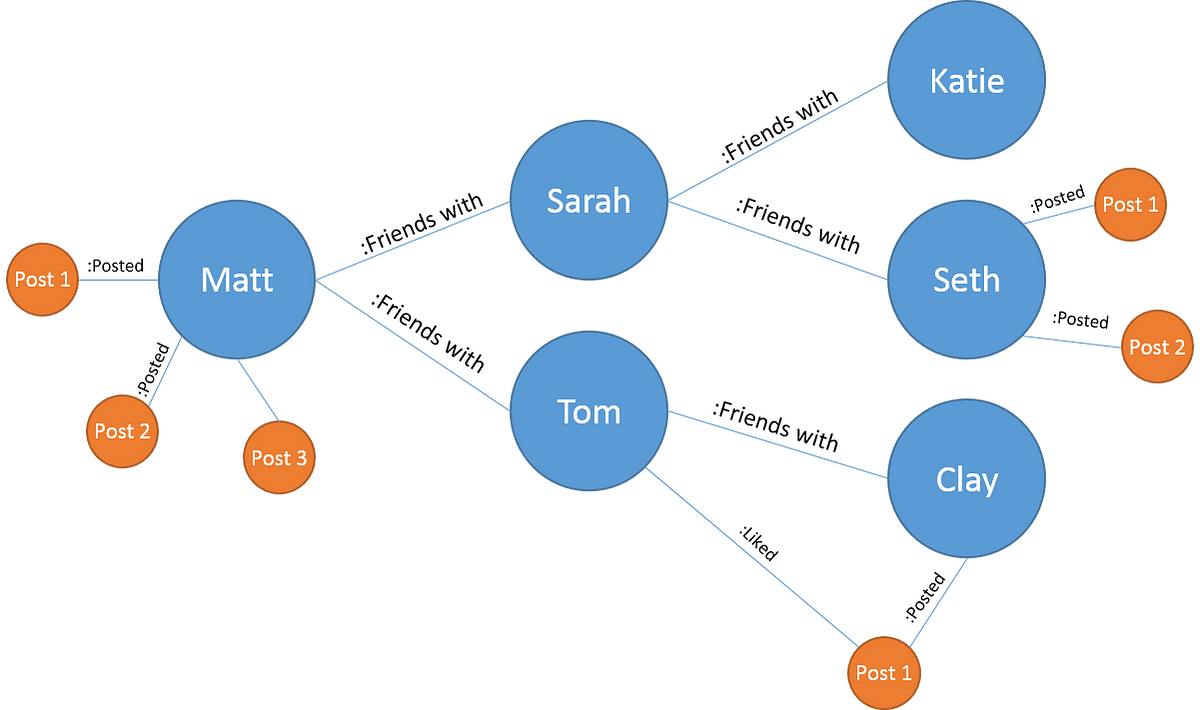
\includegraphics[width=0.7\textwidth]{images/Neo4j_graph.png}
\end{center}

\subsubsection{Neo4j}

\begin{center}
  
\includegraphics[width=0.3\textwidth]{images/Neo4j.png}
\end{center}

Neo4j es una base de datos de grafos que almacena datos en grafos. Fue creada en 2007 por Neo Technology. Su objetivo principal es ofrecer alta velocidad y escalabilidad.

\section{Teorema CAP}
El teorema CAP establece que un sistema distribuido no puede garantizar simultáneamente:

\begin{itemize}
    \item \textbf{Consistency} (Consistencia): Todos los nodos ven los mismos datos al mismo tiempo
    \item \textbf{Availability} (Disponibilidad): Cada petición recibe una respuesta
    \item \textbf{Partition Tolerance} (Tolerancia a particiones): El sistema continúa funcionando a pesar de fallos en la red
\end{itemize}

\begin{center}
\begin{tabular}{lll}
\toprule
Base de Datos & Prioriza & Sacrifica \\
\midrule
MongoDB & CP & Availability \\
Cassandra & AP & Consistency \\
Redis & CP & Availability \\
Neo4j & CA & Partition Tolerance \\
\bottomrule
\end{tabular}
\end{center}

\textbf{Nota}: MongoDB es configurable para priorizar Consistency o Availability (modo CP o modo AP, por defecto es CP). Neo4J no tolera particiones.


\section{Cuándo Usar NoSQL}
\begin{itemize}
    \item \textbf{Datos no estructurados}: Cuando los datos no tienen un esquema fijo
    \item \textbf{Escalabilidad horizontal}: Necesidad de escalar añadiendo servidores
    \item \textbf{Alta velocidad}: Requerimientos de lectura/escritura muy rápidos
    \item \textbf{Agilidad}: Desarrollo rápido con esquemas flexibles
    \item \textbf{Grandes volúmenes}: Manejo de Big Data
\end{itemize}

\section{Cuándo NO Usar NoSQL}
\begin{itemize}
    \item \textbf{Datos altamente relacionales}: Muchas relaciones complejas entre entidades
    \item \textbf{Transacciones ACID}: Necesidad de garantías ACID estrictas
    \item \textbf{Reportes complejos}: Consultas complejas con múltiples JOINs
    \item \textbf{Equipos sin experiencia}: Curva de aprendizaje significativa
\end{itemize}

\end{document}
